\begin{refsection}


\chapter{Detrital geochronology}\label{ch:detrital}

\section{Maximum depositional age estimation}

Detrital geochronology is often the only way to estimate the
depositional age of siliclastic rocks in the absence of fossils or
volcanic ash layers. Detrital zircon U--Pb geochronology in particular
has become a popular technique to obtain maximum depositional ages
(MDAs). However other chronometers such as
\textsuperscript{40}Ar/\textsuperscript{39}Ar can be used for this
purpose as well, and can in fact be more useful than U--Pb. Numerous
MDA estimation algorithms have been proposed over the years, such as:

\begin{enumerate}
\item the youngest single grain (YSG);
\item the youngest grain cluster at $1\sigma$ (YGC1$\sigma$) or
  $2\sigma$ (YGC2$\sigma$);
\item the youngest detrital zircon estimated by \citet{ludwig2003}'s
  Monte Carlo resampling algorithm (YDZ);
\item the outcome of \citet{ludwig2002}'s TuffZirc algorithm;
\item the weighted mean of the youngest three (Y3Z) or four (Y4Z)
  zircons;
\item the minimum age of grains selected by \citet{gehrels2003}'s
  AgePick algorithm.
\item the mode of the youngest graphical peak on a probability density
  plot (YPP);
\item the weighted mean of the grains in the youngest peak of a
  probability density plot ($\tau$); and
\end{enumerate}

The first six groups of methods gradually drift to younger ages with
increasing sample size, for reasons that are essentially captured by
Figure~\ref{fig:increasingn}: increasing sample size increases the
`power' of statistical tests to subdivide a population of values in to
smaller subpopulations. The youngest of these subpopulations
inevitably gets younger as the number of subpopulations increases.  In
contrast, the last two methods converged to ages that are
systematically too old. The failure of YPP and $\tau$ to retrieve the
correct depositional age reflects the underlying flaws of the
probability density plots (PDPs) on which they are based. The
shortcomings of PDPs were explained in Section~\ref{sec:KDE+CAD} and
won't be discussed further here.\\

The minimum age model of Equation~\ref{eq:Lminagemod} does not suffer
from this undesirable sample size dependency. With increasing sample
size, this model converges to a sensible value, provided that the
following assumptions are met:

\begin{enumerate}
\item the true age distribution approximately follows the functional
  form shown in Figure~\ref{fig:minagemod}; and
\item the analytical uncertainties are well characterised.
\end{enumerate}

The first assumption is generally easy to verify. If the young end of
the age spectrum is marked by a cluster of nearly concordant ages,
then the minimum age model will appropriately average these. And it
will do so even if the old end of the spectrum does not look like a
(log)normal distribution. It is not uncommon for detrital zircon U--Pb
age distributions to be fat tailed at both ends of the
spectrum. However, similar results are obtained by the full model
(Equation~\ref{eq:Lminagemod}) and a 3-parameter simplification in
which $\gamma=\mu$. This suggests that even quite strong violations of
the parametric assumptions do not have a major effect on the
outcomes.\\

If the age difference between the youngest and the second youngest
grains in a sample is significantly greater than their respective
analytical uncertainties, then the minimum age model will simply
return the youngest age as a result. In other words, for fat tailed
age spectra, the minimum age model reduces to the YSG model. This is
the most sensible solution from a statistical point of view. In the
absence of a discrete youngest age peak, the objections to the YSG
model raised before do not apply. However whether age of the youngest
grain is also the most sensible solution from a geological point of
view is a different matter.

\begin{center}
\noindent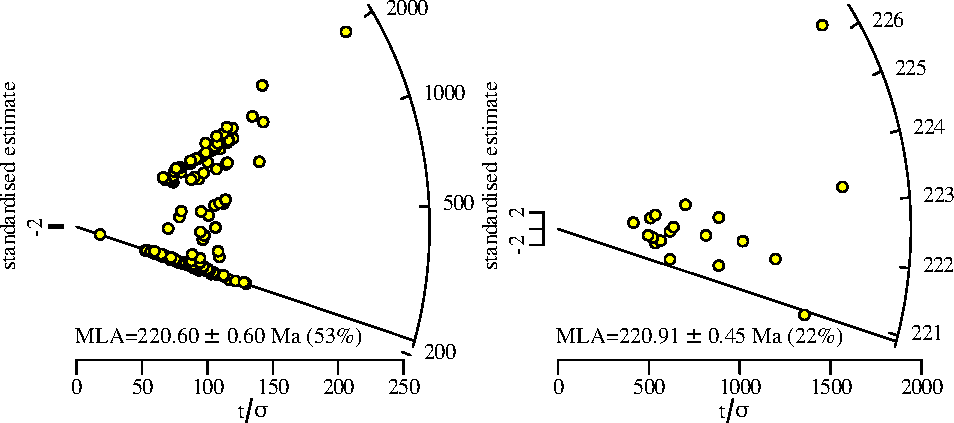
\includegraphics[width=\linewidth]{../figures/297.pdf}
\captionof{figure}{Radial plots and MDA estimates for sample 297 of
  \citet[][LA-ICPMS data, left]{gehrels2020} and \citet[][CA-TIMS
    data, right]{rasmussen2020}, calculated with \texttt{IsoplotR}
  \citep{vermeesch2018b}.  The MDA estimates agree to within 0.6\%
  despite the great differences in sample size and analytical
  precision between the two datasets. The ad hoc MDA estimation
  algorithms listed at the start of this Section do not fare so well,
  resulting in differences of 2 -- 17\% between the LA-ICPMS and
  CA-TIMS data.}
  \label{fig:297}
\end{center}

\section{Multi-sample plots}

The principal aim of the methods and graphical devices discussed thus
far has been to extract geologically meaningful information from
multiple aliquots of a single sample. However, most geochronological
applications nowadays involve multiple samples, and the differences
between these samples often has greater scientific significance than
any individual date.  \texttt{IsoplotR} implements a number of
graphical devices to facilitate the interpretation of such
multi-sample datasets. The CAD is the easiest way to simultaneously
visualise multiple age distributions on a single plot.

\noindent\begin{minipage}[t][][b]{.55\linewidth}
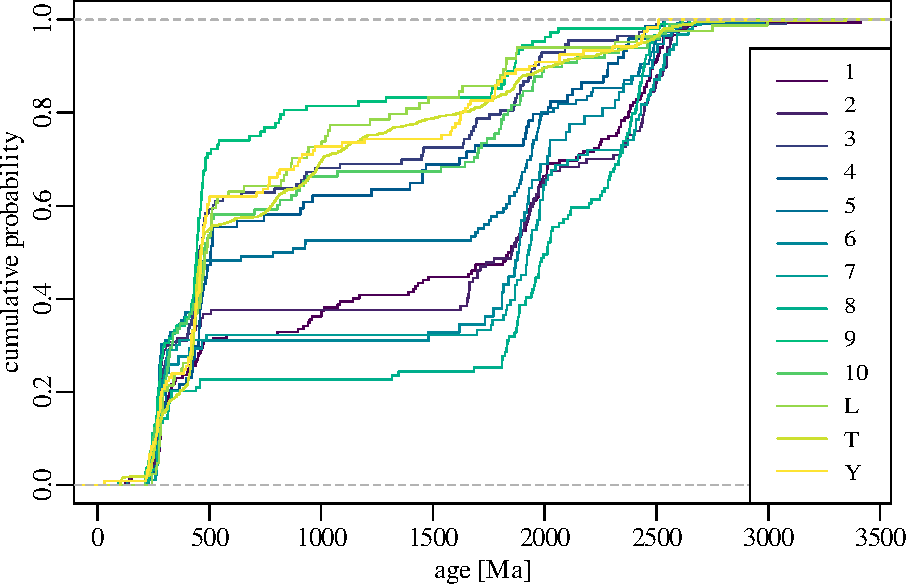
\includegraphics[width=\textwidth]{../figures/multicad.pdf}\\
\end{minipage}
\begin{minipage}[t][][t]{.45\linewidth}
  \captionof{figure}{CAD plot of 13 detrital zircon U--Pb datasets
    from China \citep{vermeesch2013}.  Samples with similar age
    distributions have CADs that plot close together. Dissimilar
    samples are characterised by greater vertical separation of their
    respective CADs. The CAD is the only way to plot several complete
    datasets together on a single panel figure.  However this plot
    becomes cluttered when used to display more than 10 or so
    samples.\\}
  \label{fig:multicad}
\end{minipage}

In contrast, KDEs are better presented in a multi-panel format. To
facilitate the intercomparison of multiple age distributions,
\texttt{IsoplotR} offers the option to force all panels to use the
same kernel bandwidth, to normalise the area under each KDE to a
common value, and to plot them all on the same timescale.\\

\noindent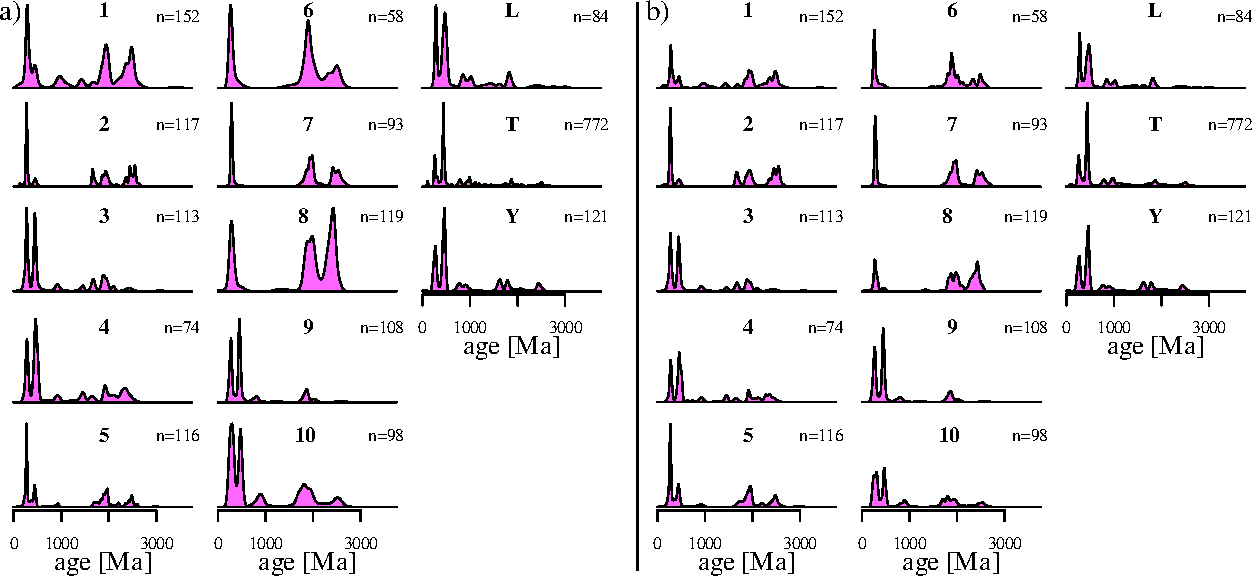
\includegraphics[width=\linewidth]{../figures/multikde.pdf}
\begingroup\captionof{figure}{ a) KDEs of the Chinese zircon data
  using different kernel bandwidths and scaled independently so as to
  display each sample to its maximimum possible extent; b) KDEs of the
  same data using the same bandwidth (the median of all the plots in
  panel a) and normalised to the same area.\\}
\label{fig:multikde}
\endgroup

Visual comparison of CADs or KDEs can be an effective way to spot
general trends and groupings in simple datasets. But this approach
becomes impractical when the inter-sample differences are subtle or
the datasets are large ($>10$ samples, say). Such cases call for an
additional layer of statistical simplification to emphasise the
geologically significant differences whilst removing the less
informative similarities. Multi-dimensional scaling (MDS) is one way
to achieve this goal.

\section{Multidimensional scaling}\label{sec:MDS}

Multidimensional Scaling (MDS) is a multivariate \textbf{ordination}
technique that is similar in many ways to PCA. MDS aims to extract two
(or higher) dimensional `maps' from tables of pairwise distances
between objects. Let us illustrate the method with a simple
geographical example. Consider the following table of pairwise
distances between European cities:

\begin{center}
  \begin{tabular}{c|ccccccc}
  &  Athens & Barcelona & Brussels & $\ldots$ & Rome & Stockholm & Vienna \\ \hline
Athens & 0 & 3313 & 2963 & $\ldots$ & 817 & 3927 & 1991 \\
Barcelona & 3313 & 0 & 1326 & $\ldots$ & 1460 & 2868 & 1802 \\
Brussels & 2963 & 1318 & 0 & $\ldots$ & 1511 & 1616 & 1175 \\
$\vdots$ & $\vdots$ & $\vdots$ & $\vdots$ & $\ddots$ &
$\vdots$  & $\vdots$ & $\vdots$ \\
Rome & 817 & 1460 & 1511 & $\ldots$ & 0 & 2707 & 1209 \\
Stockholm & 3927 & 2868 & 1616 & $\ldots$ & 2707 & 0 & 2105 \\
Vienna & 1991 & 1802 & 1175 & $\ldots$ & 1209 & 2105 & 0 
  \end{tabular}
  \captionof{figure}{Table of road distances (in km) between European
    cities. The full dataset comprises 21 cities.}
  \label{tab:eurodist}
\end{center}

Given a table of this form, MDS reconstructs the map of Europe:

\noindent\begin{minipage}[t][][b]{.4\textwidth}
  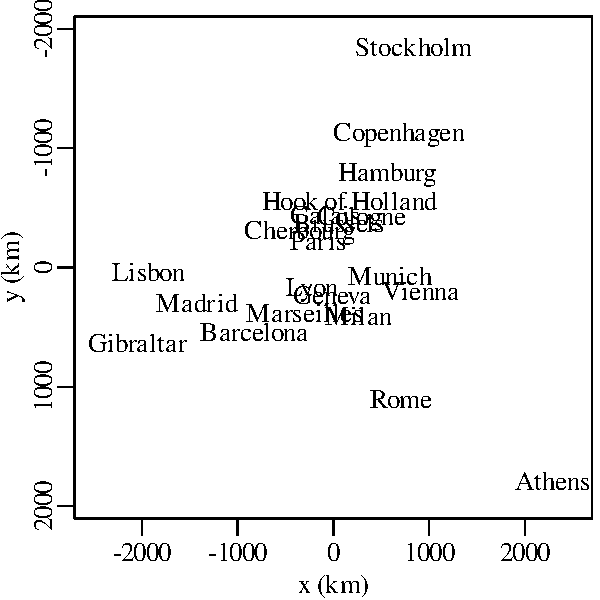
\includegraphics[width=\textwidth]{../figures/eurodist.pdf}\\
\end{minipage}
\begin{minipage}[t][][t]{.6\textwidth}
  \captionof{table}{MDS configuration of the European city distance
    data (Table~\ref{tab:eurodist}). Cities (such as Lyon and Geneva)
    that are close together in the real world plot close together on
    the MDS configuration. And cities (such as Stockholm and Athens)
    that are far apart in the real world plot on opposite ends of the
    MDS configuration. But whilst the MDS configuration preserves the
    distances, it does not preserve the orientation of the cities. In
    this figure, the y-axis has been flipped, and the city locations
    are rotated $\sim 15^\circ$ in a clockwise sense compared to the
    real map of Europe.\\}
  \label{fig:eurodist}
\end{minipage}

We can measure the distances between the cities on the MDS map (in cm,
inches or any other unit) and plot them against the input distances
(in km) from Table~\ref{tab:eurodist}. This produces a so-called
\textbf{Shepard plot}:

\noindent\begin{minipage}[t][][b]{.3\textwidth}
  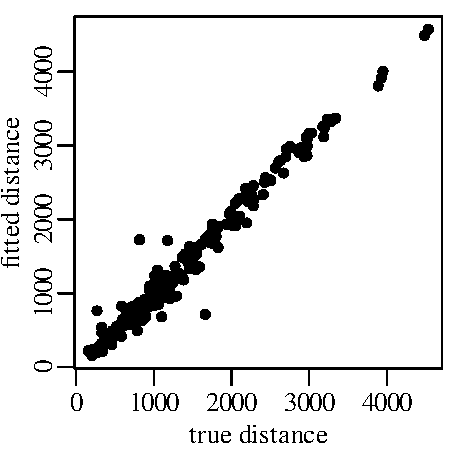
\includegraphics[width=\textwidth]{../figures/Shepard.pdf}\\
\end{minipage}
\begin{minipage}[t][][t]{.7\textwidth}
  \captionof{figure}{The Shepard plot of the European city distances
    shows a good agreement between the true input distances from
    Table~\ref{tab:eurodist} (x-axis) and the fitted distances
    measured on the MDS configuration of Figure~\ref{fig:eurodist}
    (y-axis). There are 21 cities in the dataset, resulting in
    $21\times{20}/2=210$ pairwise distances. Hence there are 210 data
    points on this scatter plot. Most of the scatter of the data
    around the best fit line is caused by the fact that the input data
    are \emph{road distances}, which do not perfectly agree with the
    straight line map distances.\\}
  \label{fig:Shepard}
\end{minipage}

The scatter of the fitted data relative to the true distances can be
quantified as the \textbf{Stress}:
\begin{equation}
  S = \sqrt{\frac{\sum_{i=1}^{n}\sum_{j=i+1}^{n}(f(d[i,j])-\delta[i,j])^2}
    {\sum_{i=1}^{n}\sum_{j=i+1}^{n}\delta[i,j]^2}}
  \label{eq:stress}
\end{equation}

\noindent where $d[i,j]$ is the input distance between objects $i$ and
$j$ (for example the Euclidean distance of Table~\ref{fig:eurodist}),
$\delta[i,j]$ is the fitted distance measured on the MDS
configuration, and $f$ is a monotonic transformation that essentially
maps $d[i,j]$ to the same scale as $\delta[i,j]$.  The European city
distance dataset is characterised by a Stress values of 7.5\%, which
corresponds to a `good' fit:
\begin{center}
  \begin{tabular}{c|ccccc}
    fit & poor & fair & good & excellent & perfect \\
    S & 0.2 & 0.1 & 0.05 & 0.025 & 0
  \end{tabular}
  \captionof{table}{Rule of thumb for interpreting the goodness of fit
    of an MDS configuration.}
  \label{tab:S}
\end{center}

The preceding paragraphs have discussed the graphical output of MDS,
but did not explain how this output is produced. It turns out that
there are several ways to do so. In its simplest form
(\textbf{classical MDS}), MDS consists of a simple sequence of matrix
operations that are similar in many ways to the widely used principal
component analysis algorithm. An alternative and more widely used
approach (\textbf{nonmetric MDS}) uses an iterative gradient search
algorithm to minimise Equation~\ref{eq:stress}.\\

Nonmetric MDS is more flexible than classical MDS because it
accommodates unconventional `dissimilarity' measures that do not
necessarily have to behave like conventional distances. So instead of
physical distances expressed in kilometres or miles, we can also use
MDS to interpret differences in chemical concentration, density,
degree of correlation, and many other numerical quantities.  In the
context of detrital geochronology, the dissimilarity between samples
is given by the statistical distance between age distributions. There
are many ways to define this statistical distance. \texttt{IsoplotR}
uses the Kolmogorov-Smirnov (KS) statistic due to its simplicity and
the fact that it behaves like a true distance in the mathematical
sense of the word \citep{vermeesch2013, vermeesch2018b}.\\

The Kolmogorov-Smirnov statistic is defined as the maximum vertical
distance between the CADs of the two samples:
\begin{equation}
  D = \underset{z}{\mbox{max}} |F_x(z) - F_y(z)|
  \label{eq:KS}
\end{equation}

\noindent where $F_x$ and $F_y$ are the CADs of $x$ and $y$,
respectively.  $D$ takes on values from 0 (two identical
distributions) and 1 (no overlap between the two distributions). To
illustrate the Kolmogorov-Smirnov method, consider two sand samples
from China: one sample from the Yellow River, and one sample from a
sand dune in the Mu Us desert:

\noindent\begin{minipage}[t][][b]{.4\textwidth}
  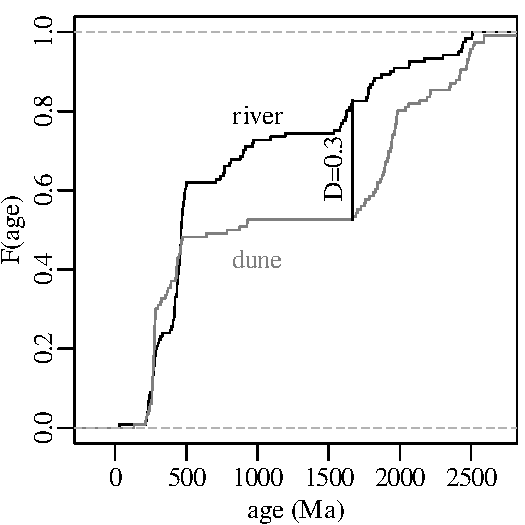
\includegraphics[width=\textwidth]{../figures/KS.pdf}\\
\end{minipage}
\begin{minipage}[t][][t]{.6\textwidth}
  \captionof{figure}{The two-sample Kolmogorov-Smirnov statistic is
    the maximum vertical distance between two CADs. This example
    compares the cumulative distributions of 121 detrital zircon U--Pb
    ages from the Yellow River with 116 detrital zircon U--Pb ages
    from a sand dune in the adjacent Mu Us desert. The KS-distance is
    0.3006.}
  \label{fig:KS}
\end{minipage}

Calculating the KS-distance between samples two at a time populates a
symmetric dissimilarity matrix with positive values and a zero
diagonal. For the Chinese dataset, this produces the following
$13\times{13}$ matrix:
\begin{equation}
  d = 
  \bbordermatrix{  & 1 & 2 & 3 & 4 & \boxed{5} &
    6 & 7 & 8 & 9 & 10 & L & T & \boxed{Y} \cr
    1 & 0 & 14 & 33 & 27 & 18 & 14 & 15 & 22 & 48 & 32 & 42 & 37 & 40 \cr
    2 & 14 & 0 & 36 & 33 & 16 & 14 & 15 & 24 & 46 & 32 & 47 & 42 & 43 \cr
    3 & 33 & 36 & 0 & 19 & 24 & 44 & 47 & 55 & 17 & 10 & 13 & 12 & 8 \cr
    4 & 27 & 33 & 19 & 0 & 20 & 38 & 41 & 48 & 28 & 14 & 21 & 17 & 16 \cr
    \boxed{5} & 18 & 16 & 24 & 20 & 0 & 22 & 24 & 33 & 31 & 20 & 33 & 28 & \boxed{30} \cr
    6 & 14 & 14 & 44 & 38 & 22 & 0 & 14 & 24 & 52 & 41 & 52 & 48 & 49 \cr
    7 & 15 & 15 & 47 & 41 & 24 & 14 & 0 & 16 & 51 & 43 & 54 & 49 & 52 \cr
    8 & 22 & 24 & 55 & 48 & 33 & 24 & 16 & 0 & 61 & 53 & 63 & 59 & 62 \cr
    9 & 48 & 46 & 17 & 28 & 31 & 52 & 51 & 61 & 0 & 20 & 22 & 18 & 16 \cr
    10 & 32 & 32 & 10 & 14 & 20 & 41 & 43 & 53 & 20 & 0 & 17 & 15 & 13 \cr
    L & 42 & 47 & 13 & 21 & 33 & 52 & 54 & 63 & 22 & 17 & 0 & 10 & 11 \cr
    T & 37 & 42 & 12 & 17 & 28 & 48 & 49 & 59 & 18 & 15 & 10 & 0 & 7 \cr
    \boxed{Y} & 40 & 43 & 8 & 16 & \boxed{30} & 49 & 52 & 62 & 16 & 13 & 11 & 7 & 0 
  }
  \label{eq:DZd}
\end{equation}

\noindent where the K-S values have been multiplied with 100 to remove
the decimal points. Square boxes mark the two samples shown in
Figure~\ref{fig:KS}. Equation~\ref{eq:DZd} is a symmetric matrix
containing positive values and a zero diagonal. Thus it fulfils all
the requirements for MDS analysis:

\noindent\begin{minipage}[t][][b]{.45\textwidth}
  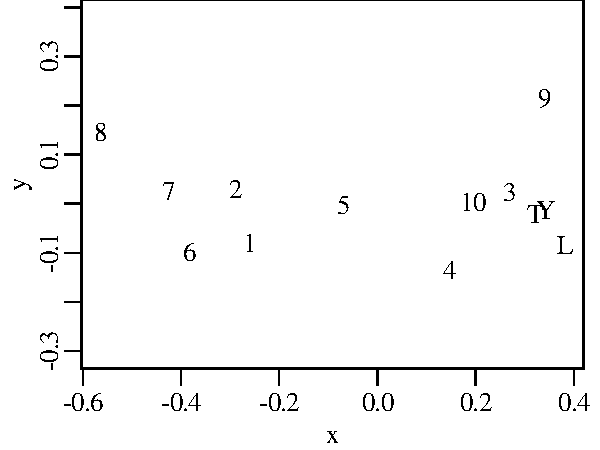
\includegraphics[width=\textwidth]{../figures/DZmds.pdf}\\
\end{minipage}
\begin{minipage}[t][][t]{.55\textwidth}
  \captionof{figure}{MDS configuration of the detrital zircon U--Pb
    data.  Samples that have similar age distributions (such as `Y'
    and `T') are characterised by low K-S statistics (e.g.,
    $d[Y,T]=0.07$) and plot close together. Samples that have greatly
    differing age distributions (such as `Y' and `8') are
    characterised by high K-S statistics (e.g., $d[Y,5]=0.62$) and
    plot far apart on the MDS map.\\}
  \label{fig:DZmds}
\end{minipage}

One simple but effective way to aid in the interpretation of MDS maps
is to draw a solid line from each point in the configuration to its
`closest' neighbour in dissimilarity-space, and a dotted line to the
second closest neighbour:

\noindent\begin{minipage}[t][][b]{.45\textwidth}
  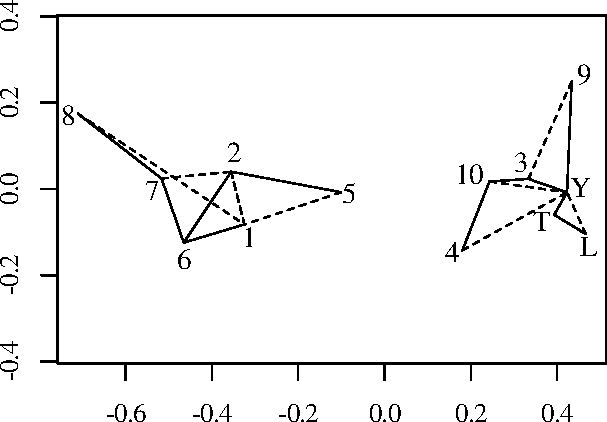
\includegraphics[width=\textwidth]{../figures/DZmds_nnlines.pdf}\\
\end{minipage}
\begin{minipage}[t][][t]{.55\textwidth}
  \captionof{figure}{ For example, sample~8 is the closest (or `least
    dissimilar') to sample~7 (D=0.16), and the second closest to
    sample~1 (D=0.22), while sample~7 is the closest to sample~6
    (D=0.14) and second closest to sample~2 (D=0.15). These connecting
    lines define two distinct groups dividing the field area into a
    southwestern area containing sediments of `Yellow River affinity'
    (samples~3, 4, 9, 10, L, T and Y) and a northeastern area
    containing sediments of a different origin (samples 1, 2, 5, 6, 7
    and 8).}
  \label{fig:DZmds_nnlines}
\end{minipage}

\printbibliography[heading=subbibliography]

\end{refsection}
